%!TEX TS-program = xelatex
\documentclass[12pt, a4paper, oneside]{article}

% пакеты для математики
\usepackage{amsmath,amsfonts,amssymb,amsthm,mathtools}  
\mathtoolsset{showonlyrefs=true}  % Показывать номера только у тех формул, на которые есть \eqref{} в тексте.

\usepackage[english, russian]{babel} % выбор языка для документа
% \usepackage[utf8]{inputenc}          % utf8 кодировка

% Основные шрифты 
\usepackage{fontspec}         
\setmainfont{Linux Libertine O}  % задаёт основной шрифт документа

% Математические шрифты 
\usepackage{unicode-math}     
\setmathfont[math-style=upright]{[Neo Euler.otf]} 


%%%%%%%%%% Работа с картинками и таблицами %%%%%%%%%%
\usepackage{graphicx} % Для вставки рисунков                
\usepackage{graphics}
\graphicspath{{images/}{pictures/}}   % папки с картинками

\usepackage{wrapfig}    % обтекание рисунков и таблиц текстом

\usepackage{booktabs}   % таблицы как в годных книгах
\usepackage{tabularx}   % новые типы колонок
\usepackage{tabulary}   % и ещё новые типы колонок
\usepackage{float}      % возможность позиционировать объекты в нужном месте
\renewcommand{\arraystretch}{1.2}  % больше расстояние между строками


%%%%%%%%%% Графики и рисование %%%%%%%%%%
\usepackage{tikz, pgfplots}  % языки для графики
\pgfplotsset{compat=1.16}

\usepackage{todonotes} % для вставки в документ заметок о том, что осталось сделать
% \todo{Здесь надо коэффициенты исправить}
% \missingfigure{Здесь будет Последний день Помпеи}
% \listoftodos --- печатает все поставленные \todo'шки


%%%%%%%%%% Внешний вид страницы %%%%%%%%%%

\usepackage[paper=a4paper, top=20mm, bottom=15mm,left=20mm,right=15mm]{geometry}
\usepackage{indentfirst}    % установка отступа в первом абзаце главы

\usepackage{setspace}
\setstretch{1.15}  % межстрочный интервал
\setlength{\parskip}{4mm}   % Расстояние между абзацами
% Разные длины в LaTeX: https://en.wikibooks.org/wiki/LaTeX/Lengths

% свешиваем пунктуацию
% теперь знаки пунктуации могут вылезать за правую границу текста, при этом текст выглядит ровнее
\usepackage{microtype}

% \flushbottom                            % Эта команда заставляет LaTeX чуть растягивать строки, чтобы получить идеально прямоугольную страницу
\righthyphenmin=2                       % Разрешение переноса двух и более символов
\widowpenalty=300                     % Небольшое наказание за вдовствующую строку (одна строка абзаца на этой странице, остальное --- на следующей)
\clubpenalty=3000                     % Приличное наказание за сиротствующую строку (омерзительно висящая одинокая строка в начале страницы)
\tolerance=10000     % Ещё какое-то наказание.

% мои цвета https://www.artlebedev.ru/colors/
\definecolor{titleblue}{rgb}{0.2,0.4,0.6} 
\definecolor{blue}{rgb}{0.2,0.4,0.6} 
\definecolor{red}{rgb}{1,0,0.2} 
\definecolor{green}{rgb}{0,0.6,0} 
\definecolor{purp}{rgb}{0.4,0,0.8} 

% цвета из geogebra 
\definecolor{litebrown}{rgb}{0.6,0.2,0}
\definecolor{darkbrown}{rgb}{0.75,0.75,0.75}

% Гиперссылки
\usepackage{xcolor}   % разные цвета

\usepackage{hyperref}
\hypersetup{
	unicode=true,           % позволяет использовать юникодные символы
	colorlinks=true,       	% true - цветные ссылки
	urlcolor=blue,          % цвет ссылки на url
	linkcolor=red,          % внутренние ссылки
	citecolor=green,        % на библиографию
	breaklinks              % если ссылка не умещается в одну строку, разбивать её на две части?
}

% меняю оформление секций 
\usepackage{titlesec}
\usepackage{sectsty}

% меняю цвет на синий
\sectionfont{\color{titleblue}}
\subsectionfont{\color{titleblue}}

% выбрасываю нумерацию страниц и колонтитулы 
\pagestyle{empty}

% синие круглые бульпоинты в списках itemize 
\usepackage{enumitem}

\definecolor{itemizeblue}{rgb}{0, 0.45, 0.70}

\newcommand*{\MyPoint}{\tikz \draw [baseline, fill=itemizeblue, draw=blue] circle (2.5pt);}

\renewcommand{\labelitemi}{\MyPoint}

% расстояние в списках
\setlist[itemize]{parsep=0.4em,itemsep=0em,topsep=0ex}
\setlist[enumerate]{parsep=0.4em,itemsep=0em,topsep=0ex}


%%%%%%%%%% Свои команды %%%%%%%%%%

% Математические операторы первой необходимости:
\DeclareMathOperator{\sgn}{sign}
\DeclareMathOperator*{\argmin}{arg\,min}
\DeclareMathOperator*{\argmax}{arg\,max}
\DeclareMathOperator{\Cov}{Cov}
\DeclareMathOperator{\Var}{Var}
\DeclareMathOperator{\Corr}{Corr}
\DeclareMathOperator{\E}{\mathop{E}}
\DeclareMathOperator{\Med}{Med}
\DeclareMathOperator{\Mod}{Mod}
\DeclareMathOperator*{\plim}{plim}

% команды пореже
\newcommand{\const}{\mathrm{const}}  % const прямым начертанием
\newcommand{\iid}{\sim i.\,i.\,d.}  % ну вы поняли...
\newcommand{\fr}[2]{\ensuremath{^{#1}/_{#2}}}   % особая дробь
\newcommand{\ind}[1]{\mathbbm{1}_{\{#1\}}} % Индикатор события
\newcommand{\dx}[1]{\,\mathrm{d}#1} % для интеграла: маленький отступ и прямая d

% одеваем шапки на частые штуки
\def \hb{\hat{\beta}}
\def \hs{\hat{s}}
\def \hy{\hat{y}}
\def \hY{\hat{Y}}
\def \he{\hat{\varepsilon}}
\def \hVar{\widehat{\Var}}
\def \hCorr{\widehat{\Corr}}
\def \hCov{\widehat{\Cov}}

% Греческие буквы
\def \a{\alpha}
\def \b{\beta}
\def \t{\tau}
\def \dt{\delta}
\def \e{\varepsilon}
\def \ga{\gamma}
\def \kp{\varkappa}
\def \la{\lambda}
\def \sg{\sigma}
\def \tt{\theta}
\def \Dt{\Delta}
\def \La{\Lambda}
\def \Sg{\Sigma}
\def \Tt{\Theta}
\def \Om{\Omega}
\def \om{\omega}

% Готика
\def \mA{\mathcal{A}}
\def \mB{\mathcal{B}}
\def \mC{\mathcal{C}}
\def \mE{\mathcal{E}}
\def \mF{\mathcal{F}}
\def \mH{\mathcal{H}}
\def \mL{\mathcal{L}}
\def \mN{\mathcal{N}}
\def \mU{\mathcal{U}}
\def \mV{\mathcal{V}}
\def \mW{\mathcal{W}}

% Жирные буквы
\def \mbb{\mathbb}
\def \RR{\mbb R}
\def \NN{\mbb N}
\def \ZZ{\mbb Z}
\def \PP{\mbb{P}}
\def \QQ{\mbb Q}


%%%%%%%%%% Теоремы %%%%%%%%%%
\theoremstyle{plain} % Это стиль по умолчанию.  Есть другие стили.
\newtheorem{theorem}{Теорема}[section]
\newtheorem{result}{Следствие}[theorem]
% счётчик подчиняется теоремному, нумерация идёт по главам согласованно между собой

% убирает курсив и что-то еще наверное делает ;)
\theoremstyle{definition}         
\newtheorem*{definition}{Определение}  % нумерация не идёт вообще


%%%%%%%%%% Задачки и решения %%%%%%%%%%
\usepackage{etoolbox}    % логические операторы для своих макросов
\usepackage{environ}
\newtoggle{lecture}

\newcounter{probNum}%[section]  % счётчик для упражнений 
\NewEnviron{problem}{%
    \refstepcounter{probNum}% увеличели номер на 1 
    {\noindent \textbf{\large \color{titleblue} Упражнение~\theprobNum}  \\ \\ \BODY}
    {}%
  }

% Окружение, чтобы можно было убирать решения из pdf
\NewEnviron{solution}{%
  \iftoggle{lecture}
    {\noindent \textbf{\large Решение:} \\ \\ \BODY}
    {}%
  }
  
% выделение по тексту важных вещей
\newcommand{\indef}[1]{\textbf{ \color{green} #1}} 


\begin{document} % Конец преамбулы, начало файла

% Если переключить в false, все solution исчезнут из pdf
\toggletrue{lecture}
%\togglefalse{lecture}



\section*{Семинар 8:  Метрики классификации}

В этом семинаре мы подробнее поговорим про классификацию и метрики для неё. План будет таким: 

\begin{itemize}
	\item сформулируем задачу и поймём её специфику;
	\item поймём с помощью каких метрик можно оценить качество прогнозирования;
	\item попробуем разобраться какой смысл стоит за этими метриками.
\end{itemize}

\todo[inline]{Сюда котов и собакенов} 


\subsection*{Задача 1 (формулируем задачу)}

Вася --- меломан. Каждый день он смотрит на youtube музыкальные клипы и читает комментарии к ним. В один прекрасный день ему стало интересно, можно ли определить жанр клипа (рэп или попса) по его характеристикам: число комментов, лайков, характер комментов и тп. 

\begin{enumerate}
	\item К какому типу относится такая задача: классификация или регрессия? Почему? 
	
	\item Какие факторы из профилей вы бы использовали, чтобы её решить? Как бы вы оценивали качество итогового прогноза?
\end{enumerate}


\subsection*{Задача 2 (метрики)}

Бандерлог оценил три модели: нейросеть, случайный лес и KNN.  Он построил на тестовой выборке прогнозы и получил три матрицы ошибок: 

\begin{minipage}[t]{0.33\textwidth}
	\begin{tabular}{|c|c|c|}
		\hline
		& $y=1$  &  $ y = 0$ \\  \hline 
		$\hat y = 1$  &   $80$ &    $20$ \\      \hline 
		$\hat y = 0$ &   $20$ &     $80$ \\      \hline 
	\end{tabular}
\end{minipage}
\begin{minipage}[t]{0.33\textwidth}
	\begin{tabular}{|c|c|c|}
		\hline
		& $y=1$  &  $ y = 0$ \\  \hline 
		$\hat y = 1$  &   $48$ &    $2$ \\      \hline 
		$\hat y = 0$ &   $52$ &     $98$ \\      \hline 
	\end{tabular}
\end{minipage}
\begin{minipage}[t]{0.33\textwidth}
	\begin{tabular}{|c|c|c|}
		\hline
		& $y=1$  &  $ y = 0$ \\  \hline 
		$\hat y = 1$  &   $10$ &    $20$ \\         \hline 
		$\hat y = 0$ &   $90$ &    $10000$ \\   \hline 
	\end{tabular}
\end{minipage}

\begin{enumerate}
	\item[а)]   Найдите для всех трёх моделей долю правильных ответов. Чем плоха эта метрика? 
	\item[б)]   Найдите для всех трёх моделей точность (precision) и полноту (recall)
	\item[в)]   Предположим, что целевая переменная $y$ принимает значение $1$, если заемщик вернул кредит  и $0$, если не вернул. Вы хотите научиться прогнозировать платежеспособность клиента. Какую из первых двух моделей вы бы выбрали в таком случае? 
	\item[г)]  Предположим, что целевая переменная $y$ принимает значение $1$, если человек болен больной болезнью с болью и $0$, если он здоров. Вы хотите спрогнозировать нужно ли человеку обследование. Какую из первых двух моделей вы б выбрали в этом случае? 
\end{enumerate}

\ifbool{answers}{
	\textbf{Решение:}
	
	\begin{enumerate}
		\item[а)] 	Ежели мы совершаем ошибку, то мы делаем это спрогнозировав $\hat y = 1$ там, где реально должно быть $y = 0$ либо наоборот, прогнозируя $\hat y = 0$ там, где реально должно быть $y=1$.  В остальных случаях всё ок.  Наша классная табличка выглядит следущим образом: 
		
		\begin{center}
			\begin{tabular}{|c|c|c|}
				\hline
				& $y=1$  &  $ y = 0$ \\  \hline 
				$\hat y = 1$  &    $TP$ &     $FP$ \\      \hline 
				$\hat y = 0$ &    $FN$ &     $TN$ \\      \hline 
			\end{tabular}
		\end{center}
		
		Долю правильных ответов можно посчитать как 
		
		\[
		Accuracy = \frac{TP + TN}{TP + TN + FP + FN}.
		\]
		
		Давайте проделаем эту несложную процедуру для вердиктов всех трёх алгоритмов, описанных выше. 
		
		\begin{equation} 
		\begin{aligned}
		&Accuracy_1 = \frac{80 + 80}{80 + 80 + 20 + 20} = 0.8   \\ 
		&Accuracy_2 = \frac{48 + 98}{48 + 98 + 2 + 52} = 0.73  \\ 
		&Accuracy_3 = \frac{10 + 10000}{10 + 10000 + 20 + 90} = 0.98  \\ 
		\end{aligned}
		\end{equation} 
		
		У этой метрики есть как минимум две существенные проблемы. 
		
		Первая проблема связана с несбалансированными выборками. Именно такая ситуация наблюдается в третьей табличке. Нулевой класс заметно перетягивает на себя выборку. Выходит, что если мы просто-напросто спрогнозируем, что все объекты в выборке нулевые, мы получим табличку 
		
		\begin{center}
			\begin{tabular}{|c|c|c|}
				\hline
				& $y=1$  &  $ y = 0$ \\  \hline 
				$\hat y = 1$  &   $0$ &    $0$ \\         \hline 
				$\hat y = 0$ &   $100$ &    $10020$ \\   \hline 
			\end{tabular}
		\end{center}
		
		и $Accuracy = 0.99$. Наша модель показала более низкое качество, чем простое угадывание. Выходит, что наша модель абсолютно бесполезна. 
		
		Чтобы «бороться» с этой проблемой, используется следующий факт. Пусть $q_0$ — доля объектов самого крупного класса, тогда доля правильных ответов для разумных алгоритмов $accuracy \in [q_0,1]$, а не $[0.5, 1]$, как это можно было бы ожидать. Поэтому, если получается высокий процент правильных ответов, это может быть связано не с тем, что построен хороший классификатор, а с тем, что какого-то класса сильно больше, чем остальных.
		
		Вторая проблема с долей верных ответов состоит в том, что она никак не учитывает разные цены разных типов ошибок. Тогда как цены действительно могут быть разными.
		
		Например, представим себе линейное небо, которое бороздят вражеские самолёты. Мы стоим на земле, у нас есть пушка и снаряды. Сбивать вражеские самолёты можно руководствуясь двумя разными стратегиями: 
		
		\textbf{Путь первый:}  стрелять по всему небу, куда только можно попасть. В таком случае точность наших выстрелов будет низкой, но зато мы собьём все самолёты, то есть добьёмся высокой полноты. Такая стратегия на картинке прорисована красными лазерными выстрелами из пушки.
		
		\textbf{Путь второй:} стрелять поточнее, пореже. Тогда мы будем сбивать самолёты точно, потратим мало снарядов вхолостую, но собьём не все самолёты. Такая стратегия на картинке прорисована зелёными выстрелами из пушки. 
		
		\begin{center}
			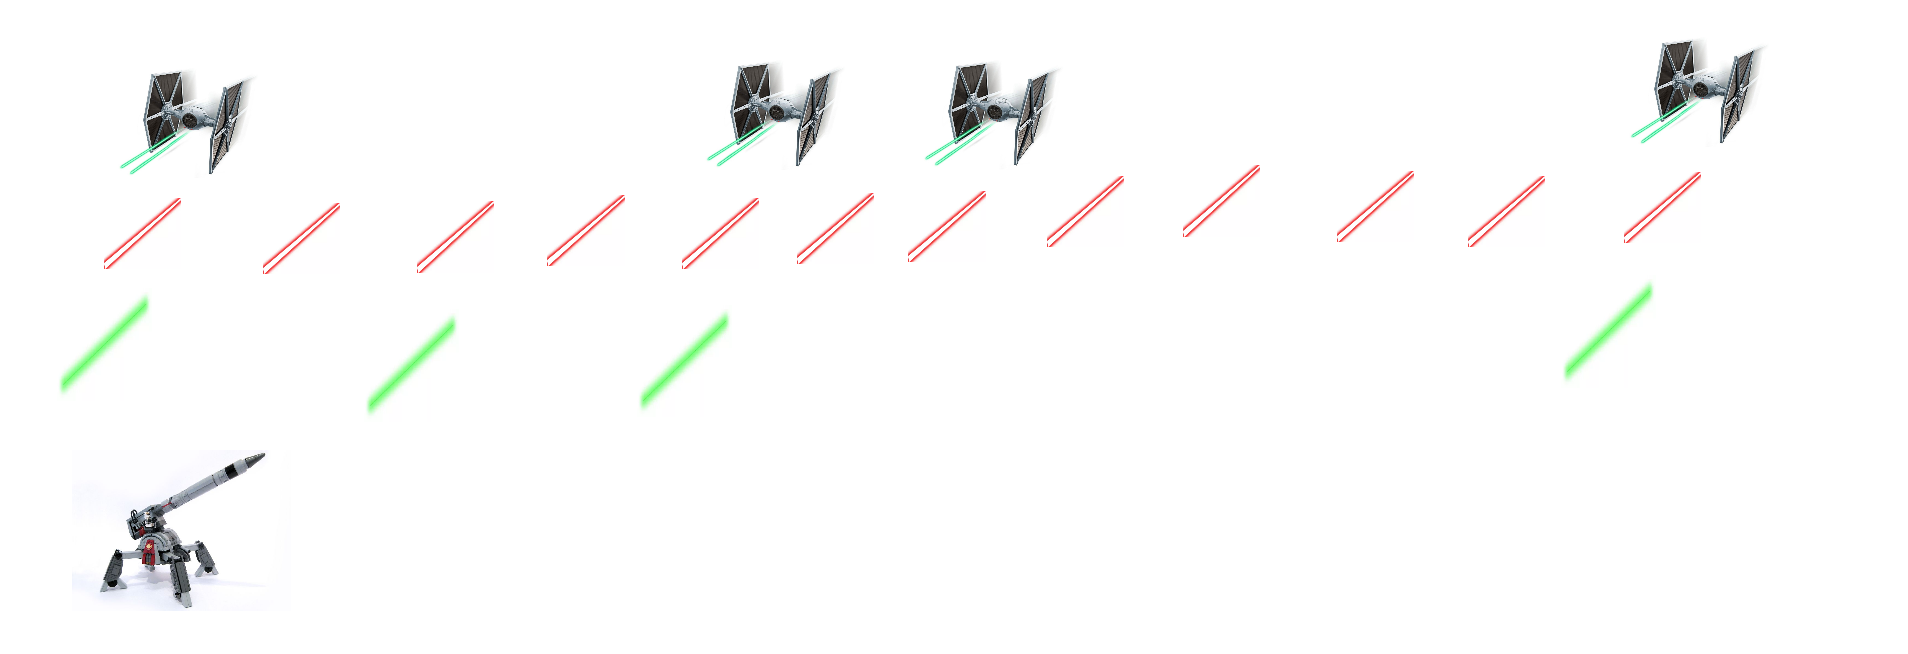
\includegraphics[width=.79\paperwidth]{fly.png}
		\end{center}
		
		
		Для разных задач бывают характерны разные стратегии. Если вернуться к нашей исходной таблице ошибок, то за точность классификатора будет отвечать первая строка
		
		\[ 
		Precision = \frac{TP}{TP + FP}.
		\]
		
		За полноту будет отвечать первы столбец
		
		\[Recall = \frac{TP}{TP + FN}.\]
		
		Посмотрим ещё один пример: если мы решаем задачу крединтого скоринга, нам нужно получить деньги назад после выдачи кредитов, иначе мы разоримся. Нам нужна модель, которая будет точно определять надёжного заёмщика. В этой ситуации для нас неважно покрыть все вражеские истребители снарядами (выдать кредиты каждому надёжному заёмщику), для нас важно сделать это точно. Поэтому основное внимание мы уделяем ошибке $FP$. 
		
		Если мы пытаемся найти больных больной болезнью с болью и отправить их делать дополнительные анализы, для нас страшнее $FN$ ошибка. Если мы отправим лишнего человека на анализы, ничего страшного с ним не произойдёт. Если мы забудем проверить больного, он умрёт. Тут лучше добиться высокой полноты, при небольшой точности. 
		
		В разных ситуациях ошибки имеют разные цены. $Accuracy$ не видит этого, поэтому на практике обычно используют $Precision$ и $Recall$. 
		
		\item[б)]  
		
		\begin{equation} 
		\begin{aligned}
		&Precision_1 =  0.8   \qquad &Recall_1 = 0.8 \\ 
		&Precision_2 = 0.96  \qquad &Recall_2 = 0.48 \\ 
		&Precision_3 = 0.33  \qquad &Recall_3 = 0.1  \\
		\end{aligned}
		\end{equation} 
		
		Вторая модель является очень точной, но в ущерб полноте. Третья модель очень плохая. Эти две метрики, в отличие от $Accuracy$, позволили заметить этот факт. 
		
		\item[в)] При использовании первой модели кредит будет выдан 100 клиентам, 80 из которых его вернут. Во второй модели, более консервативной, кредит был выдан только 50 клиентам, причем вернули его в 48 случаях. 
		
		Выше мы обсудили, что бизнес-специфика задачи диктует нам необходимость взять модель, где побольше точность.
		
		\item[г)]  Выше мы обсудили, что нам нужна модель, где побольше полнота.
	\end{enumerate}
}


\subsection*{Задача 3 (ещё немного метрик)}

Бандерлог из Лога\footnote{деревня в Кадуйском районе Вологодской области} ведёт блог, любит считать логарифмы и оценивать модели. С помощью нового алгоритма Бандерлог решил задачу классификации по трём наблюдениям и получил $b_i = \hat P(y_i = 1|x_i)$.

\begin{center}
	\begin{tabular}{c|c}
		$y_i$ & $b_i$ \\
		\hline
		$1$  & $0.7$ \\
		$0$ & $0.2$ \\
		$0$ & $0.3$ \\
		$1$ & $0.25$ \\
	\end{tabular}
\end{center}

\begin{enumerate}
	\item[a)] Найдите ROC AUC.
	\item[б)] Постройте ROC-кривую.
	\item[в)] Постройте PR-кривую (кривая точность-полнота).
	\item[г)] Найдите площадь под PR-кривой.
	\item[д)] Как по-английски будет «бревно»?
\end{enumerate}

\ifbool{answers}{
	\textbf{Решение:}
	
	\begin{enumerate}	
		\item[а)]  В предыдущей задаче мы немного обсудили метрики классификации. Когда мы на практике оцениваем модель, она выплёвывает в нас не принадлежность объекта к классу в явном виде, а вероятности того, что наши объекты --- единички. 
		
		Например, давайте думать в терминах оттока клиентов. Пусть наш сервис привлёк каких-то ребят в постоянные пользователи. Если они начнут унывать, им захочется свалить. Это называется оттоком. Давайте предположим, что модель выдаёт нам вероятность того, что человек решил приуныть. Если мы сможем понимать кто собрался приуныть, будем одаривать их ништяками и тогда они будут оставаться нашими клиентами. 
		
		Как понять, кто собирается приуныть, если модель выплёвывает на нас вероятности? Давайте выберем порог и будем считать, что все, у кого вероятность уныния $\ge 0.5$ --- отностяся к классу $1$. Есть вероятность, что они решат свалить. Их и будем одаривать ништяками. В нем случае получатся прогнозы: $1,0,0,0$. Если взять порог $0.3$, получим прогнозы $1,0,1,0$. 
		
		Как выбрать порог, кого одаривать ништяками. Если у нас большой бюджет, можно попробовать поставить низкий порог, чтобы добиться большой полноты. Если маленький бюджет, то давайте поставим порог так, чтобы борьба с унынием была поточнее. Выбор порога зависит от специфики бизнеса и от того, что от нас хотят. 
		
		Видно, что точность и полнота зависят от выбора порога. А хотелось бы, чтобы та метрика, по которой мы выбираем модель, от порога не зависила. Так рождаются идеи о метриках $roc_auc$ и $pr_auc$. 
		
		Представим себе два объекта: приунывший и нормальный. Представим себе, что модель предсказала нам вероятность уныния для первого объекта $b_1$ и для второго $b_2$.
		
		\begin{equation} 
		\begin{aligned}
		&y = 1   \qquad &\hat P(y = 1) = b_1\\ 
		&y = 0  \qquad & \hat P(y = 1) = b_2\\ 
		\end{aligned}
		\end{equation} 
		
		Если у нас хорошая модель, то явно $b_1 > b_2$. Иначе модель всё путает и говорит, что неунывающие приуныли. Давайте посмотрим как часто на нашей выборке такая путаница происходит и рассмотрим все возможные пары нулей и единичек. Всего будет четыре пары. 
		
		\begin{equation} 
		\begin{aligned}
		& 0.7 > 0.2 \qquad & ok \\
		& 0.7 > 0.3 \qquad & ok \\
		& 0.25 > 0.2 \qquad & ok \\ 
		& 0.25 < 0.3 \qquad & not \mbox{ } ok \\
		\end{aligned}
		\end{equation} 
		
		Видим, что модель ошиблась в упорядочивании один раз. $roc_auc$ --- это доля пар, где модель оказалась права. В нашем случае это $0.75$. $roc_auc$ принимает значения от $0.5$ до $1$, если её значения близки к $0.5$, наш алгоритм ничем не лучше монетки, потому что он упорядочивает пары из унывших и нормальных абы как. 
		
		Такая метрика позволяет не привязываться к конкретному значению порога и видеть насколько классно у модели выходит упорядочивать пары объектов. 
		
		\item[б)]  Величина, которую мы посчитали выше является площадью под roc-кривой (roc = receiver operating characteristic, иногда говорят «кривая ошибок»), с помощью которой часто визуализируют качество работы алгоритма.  Когда говорять про roc-auc имется в виду area under the curve. 
		
		Чтобы нарисовать ROC-кривую, надо взять единичный квадрат на координатной плоскости, разбить его на m равных частей горизонтальными линиями и на $n$ – вертикальными, где $m$ – число $1$ среди правильных меток теста (в нашем примере $m=2$), $n$ – число нулей ($n=2$). В результате квадрат разбивается сеткой на $m \times n$ блоков.
		
		Отсортируем нашу табличку по значению вероятности, которую предсказала модель. 
		
		\begin{center}
			\begin{tabular}{c|c}
				$y_i$ & $b_i$ \\
				\hline
				$1$  & $0.7$ \\
				$0$ & $0.3$ \\
				$1$ & $0.25$ \\
				$0$ & $0.2$ \\
			\end{tabular}
		\end{center}
		
		Теперь будем просматривать строки сверху вниз и прорисовывать на сетке линии, переходя их одного узла в другой. Стартуем из точки $(0, 0)$. Если значение метки класса в просматриваемой строке $1$, то делаем шаг вверх; если $0$, то делаем шаг вправо. Ясно, что в итоге мы попадём в точку $(1, 1)$, т.к. сделаем в сумме $m$ шагов вверх и $n$ шагов вправо.
		
		
		\begin{center}
			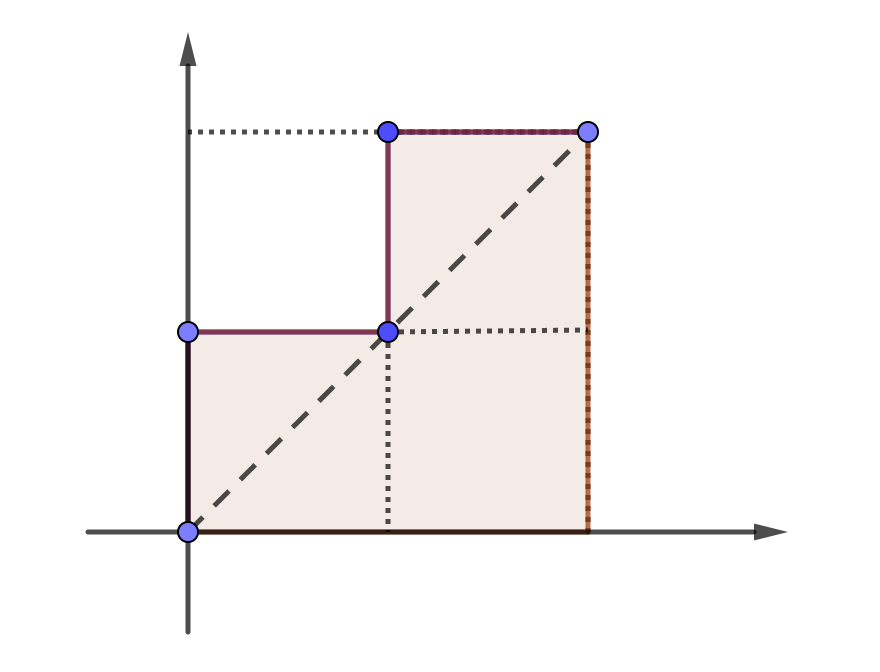
\includegraphics[width=.4\paperwidth]{roc_auc.png}
		\end{center}
		
		Сетка разбила квадрат на  $m \times n$ блоков. Ровно столько же пар вида (объект класса $1$, объект класса $0$), составленных из объектов тестовой выборки. Каждый закрашенный блок соответствует паре (объект класса $1$, объект класса $0$), для которой наш алгоритм правильно предсказал порядок (объект класса $1$ получил оценку выше, чем объект класса $0$), незакрашенный блок – паре, на которой ошибся.
		
		\item[в)] Давайте по оси $x$ откладывать полноту, а по оси $y$ точность. Давайте по очереди перебирать разные пороги и считать для них точность и полноту. Нанесём на картинку все полученные точки и соединим их. Это и будет $PR$-кривая. 
		
		Например, если мы возьмём порог $ \ge 0.2$, тогда все объекты будут принадлежать к классу $1$ точность составит $0.5$, а полнота $1$.  Если мы возьмём порог $\ge 0.25$, тогда один объект будет нулевым, а остальные три единичными.  Точность составит $0.66$, а полнота $1$.  По аналогии получим точность и полноту при порогах $\ge 0.3$ и $\ge 0.7$. 
		
		\begin{center}
			\begin{tabular}{c|c|c}
				порог &точность  & полнота\\
				\hline
				$0.2$ & $0.5$ & $1$ \\
				$0.25$ & $0.66$ & $1$ \\
				$0.3$ & $0.5$ & $0.5$ \\
				$0.7$ & $1$ & $0.5$ \\
				$0.8$ & $0$ & $0$ \\
			\end{tabular}
		\end{center}
		
		Строим кривую! 
		
		\begin{center}
			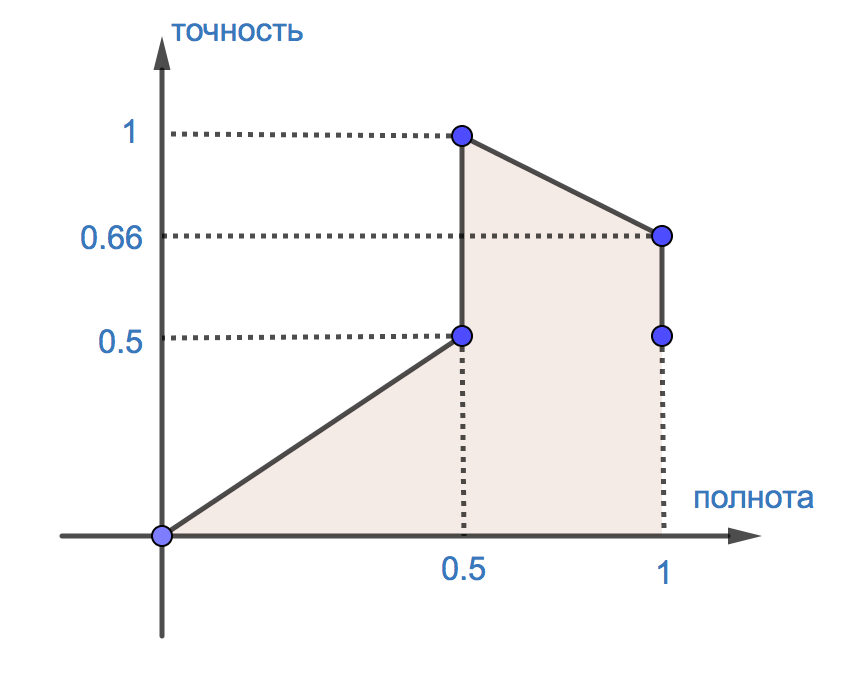
\includegraphics[width=.4\paperwidth]{pr_rc.png}
		\end{center}
		
		PR- кривая всегда начинается из точки $(0,0)$ и заканчивается в точке $(1,r)$, где $r$ --- это доля объектов первого класса в выборке. 
		
		В случае идеального классификатора, то есть если существует такой порог, что и точность, и полнота равны $100\%$, кривая будет проходить через точку $(1, 1)$. Таким образом, чем ближе кривая пройдет к этой точке, тем лучше оценки. Площадь под этой кривой может быть хорошей мерой качества оценок принадлежности к классу $1$. Такая метрика называется pr-auc, или площадь под PR-кривой.
		
		
		\item[г)] Посчитав площадь под кривой получим pr-auc.  Будем делать это, считая площади треугольников и прямоугольников. 
		
		\[
		1 - 0.5^2 - 0.5^2 \cdot 0.5 - 0.33 \cdot 0.5 \cdot 0.5 = 0.542
		\]
		
		Эта метрика подобно roc-auc не зависит от выбора порога и отражает способность модели правильно упорядочивать пары, но немножечко в другом плане.  Эта метрика строится в осях точность и полнота. Из-за этого она чувствительна к дисбалансу в классах. 
		
		Можно посмотреть на метрику roc-auc немного иначе.  Ввести две дроби
		
		\[TPR = \frac{TP}{TP +FN} \qquad FPR = \frac{FP}{FP +TN}, \]
		
		перебирать порог и в осях, соответсвующих $TPR$ и $FPR$ отмечать точки. В итоге получится ровно такая же кривая как у нас. Именно такое определение вы встретите в большинстве курсов по ML. Но любой нормальный человек сразу же забывает что означают эти $FPRFRTPRPR$, поэтому мы так делать не будем. 
		
		Единственный профит от такого определения в том, что сразу же видно, что roc-auc устройчив к дисбалансу в классах. 
		
		\item[д)]  log 
		
	\end{enumerate}
}



\section*{Ещё задачи!}

Тут лежит ещё несколько задач для самостоятельного решения. Возможно, похожие будут в самостоятельной работе... 

\subsection*{Задача 4}

Бандерлог начинает все определения со слов «это доля правильных ответов»:
\begin{enumerate}
	\item[а)] accuracy — это доля правильных ответов\ldots
	\item[б)] точность (precision) — это доля правильных ответов\ldots
	\item[в)] полнота (recall) — это доля правильных ответов\ldots
	\item[г)] TPR — это доля правильных ответов\ldots
\end{enumerate}

Закончите определения Бандерлога так, чтобы они были, хм, правильными.

\ifbool{answers}{
	\textbf{Решение:}
	
	\begin{enumerate}
		\item[а)] $\text{accuracy} = \frac{\text{TP} + \text{TN}}{\text{TP} +\text{FP} +\text{FN} +\text{TN}}$
		\item[б)] $\text{precision} = \frac{\text{TP}}{\text{TP} +\text{FP}}$
		\item[в)] $\text{recall} = \frac{\text{TP}}{\text{TP} +\text{FN}}$
		\item[г)] $\text{TPR} = \frac{\text{TP}}{\text{TP} +\text{FN}}$
	\end{enumerate}
}


\subsection*{Задача 5}

Бандерлог обучил модель для классификации и получил вектор предсказанных вероятностей принадлежностей к классу $1$. 

\begin{center}
	\begin{tabular}{c|c}
		$y_i$ & $b_i$ \\
		\hline
		$1$  & $0.9$ \\
		$0$ & $0.1$ \\
		$0$ & $0.75$ \\
		$1$ & $0.56$ \\
		$1$ & $0.2$ \\
		$0$ & $0.37$ \\
		$0$ & $0.25$ \\		
	\end{tabular}
\end{center}

\begin{enumerate}
	\item[а)]  Бинаризуйте ответ по порогу $t$ и посчитайте точность и полноту для $t = 0.3$ и для  $t = 0.8$.
	\item[б)]  Какой порог бы вы выбрали? 
	\item[в)]  Постройте ROC-кривую и найдите площадь под ней. 
\end{enumerate}


\ifbool{answers}{
	\textbf{Решение:}
	
	\begin{enumerate}
		\item[а)]  Построим в нашей табличке две колонки с прогнозами. Для удобства. 
		
		\begin{center}
			\begin{tabular}{c|c|c|c}
				$y_i$ & $b_i$ & $t=0.3$  & $t=0.8$\\
				\hline
				$1$  & $0.9$ & $1$ & $1$ \\
				$0$ & $0.1$ & $0$ & $0$\\
				$0$ & $0.75$ & $1$ & $0$\\
				$1$ & $0.56$ & $1$ & $0$\\
				$1$ & $0.2$ & $0$ & $0$ \\
				$0$ & $0.37$ & $1$ & $0$\\
				$0$ & $0.25$ & $0$ & $0$ \\		
			\end{tabular}
		\end{center}
		
		Построим для обоих порогов матрицы ошибок. Слева матрица, соответствующая порогу $0.3$, справа матрица, соответствующая порогу $0.8$.
		
		\begin{minipage}[t]{0.45\textwidth}
			\begin{tabular}{|c|c|c|}
				\hline
				& $y=1$  &  $ y = 0$ \\  \hline 
				$\hat y = 1$  &   $2$ &    $2$ \\      \hline 
				$\hat y = 0$ &   $1$ &    $2$ \\      \hline 
			\end{tabular}
		\end{minipage}
		\begin{minipage}[t]{0.45\textwidth}
			\begin{tabular}{|c|c|c|}
				\hline
				& $y=1$  &  $ y = 0$ \\  \hline 
				$\hat y = 1$  &   $1$ &    $1$ \\      \hline 
				$\hat y = 0$ &   $2$ &    $3$ \\      \hline 
			\end{tabular}
		\end{minipage}
		
		Считаем для обоих случаев точность и полноту. 
		
		\begin{equation} 
		\begin{aligned}
		&Precision_1 = 0.5     \qquad &Recall_1 = 0.66  \\ 
		&Precision_2 = 0.5  \qquad &Recall_2 =  0.33   \\ 
		\end{aligned}
		\end{equation} 
		
		\item[б)]  Обе модели дают одинаковую точность при разной полноте. У первой модели полнота повыше, имеет смысл выбрать её (но это неточно, надо бы это проверить на большем числе данных). 
		
		\item[в)] Построим roc-кривую. Для этого отсортируем все наблюдения в нашей табличке по возрастанию.
		
		\begin{center}
			\begin{tabular}{c|c}
				$y_i$ & $b_i$ \\
				\hline
				$1$  & $0.9$ \\
				$0$ & $0.75$ \\
				$1$ & $0.56$ \\
				$0$ & $0.37$ \\	
				$0$ & $0.25$ \\			
				$1$ & $0.2$ \\												
				$0$ & $0.1$ \\
			\end{tabular}
		\end{center}
		
		Заведём сетку размера 4 на 3 и начнём делать шаги по ней так, как было описано во второй задаче.
		
		\begin{center}
			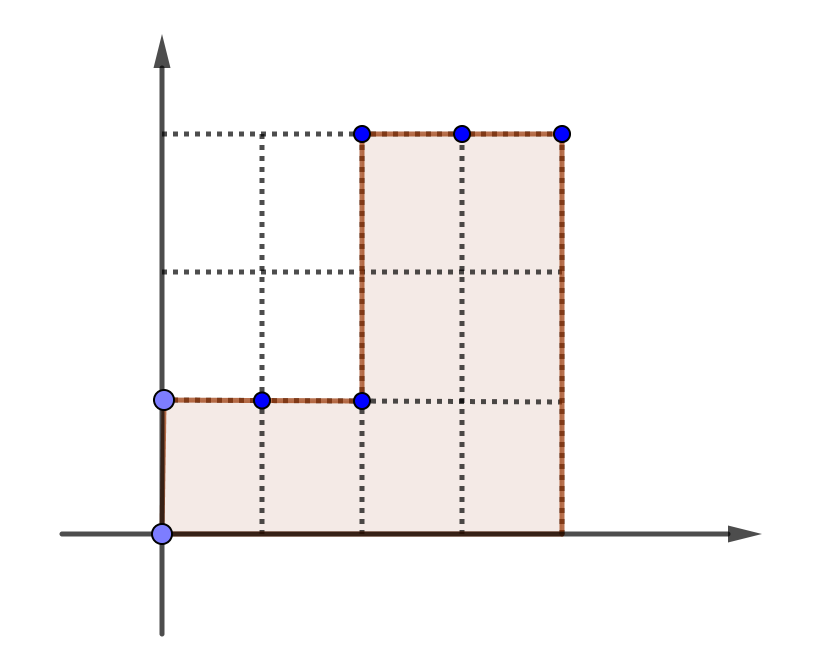
\includegraphics[width=.4\paperwidth]{roc_auc2.png}
		\end{center}
		
		Профит, получили roc-кривую.  Видим, что площадь под ней равна $\frac{8}{12}$. Иным языком говоря, среди $12$ пар ноликов и единичек, вероятности отсортированы так, как нам хотелось бы $8$ раз. 
		
		Для первого наблюдения $(1, 0.9)$ все четыре пары верны. Для второго $(1, 0.56)$ будет одна ошибочная сортировка, для третьей $(1,0.2)$ будет три ошибочных сортировки. 
	\end{enumerate}
	
}


\end{document}
